%%%%%%%%%%%%%%%%%%%%%%%%%%%%%%%%%%%%%%%%%%%%%%%%%%%%%%%%%%%%%%%%%%%%%%%%%%%%%%
\section{Degrader geometry}

The pion degrader was initially introduced to suppress the background to \piplusenu\
from muon decays in flight. It is a disk made of non-magnetic material inserted
into the beam during the calibration runs and moved out of the beam for the data taking.

\begin{figure}[H]
  \begin{tikzpicture}
    \node[anchor=south west,inner sep=0] at (0,-10.) {
      % \node[shift={(0 cm,0.cm)},inner sep=0,rotate={90}] at (0,0) {}
      \makebox[\textwidth][c] {
        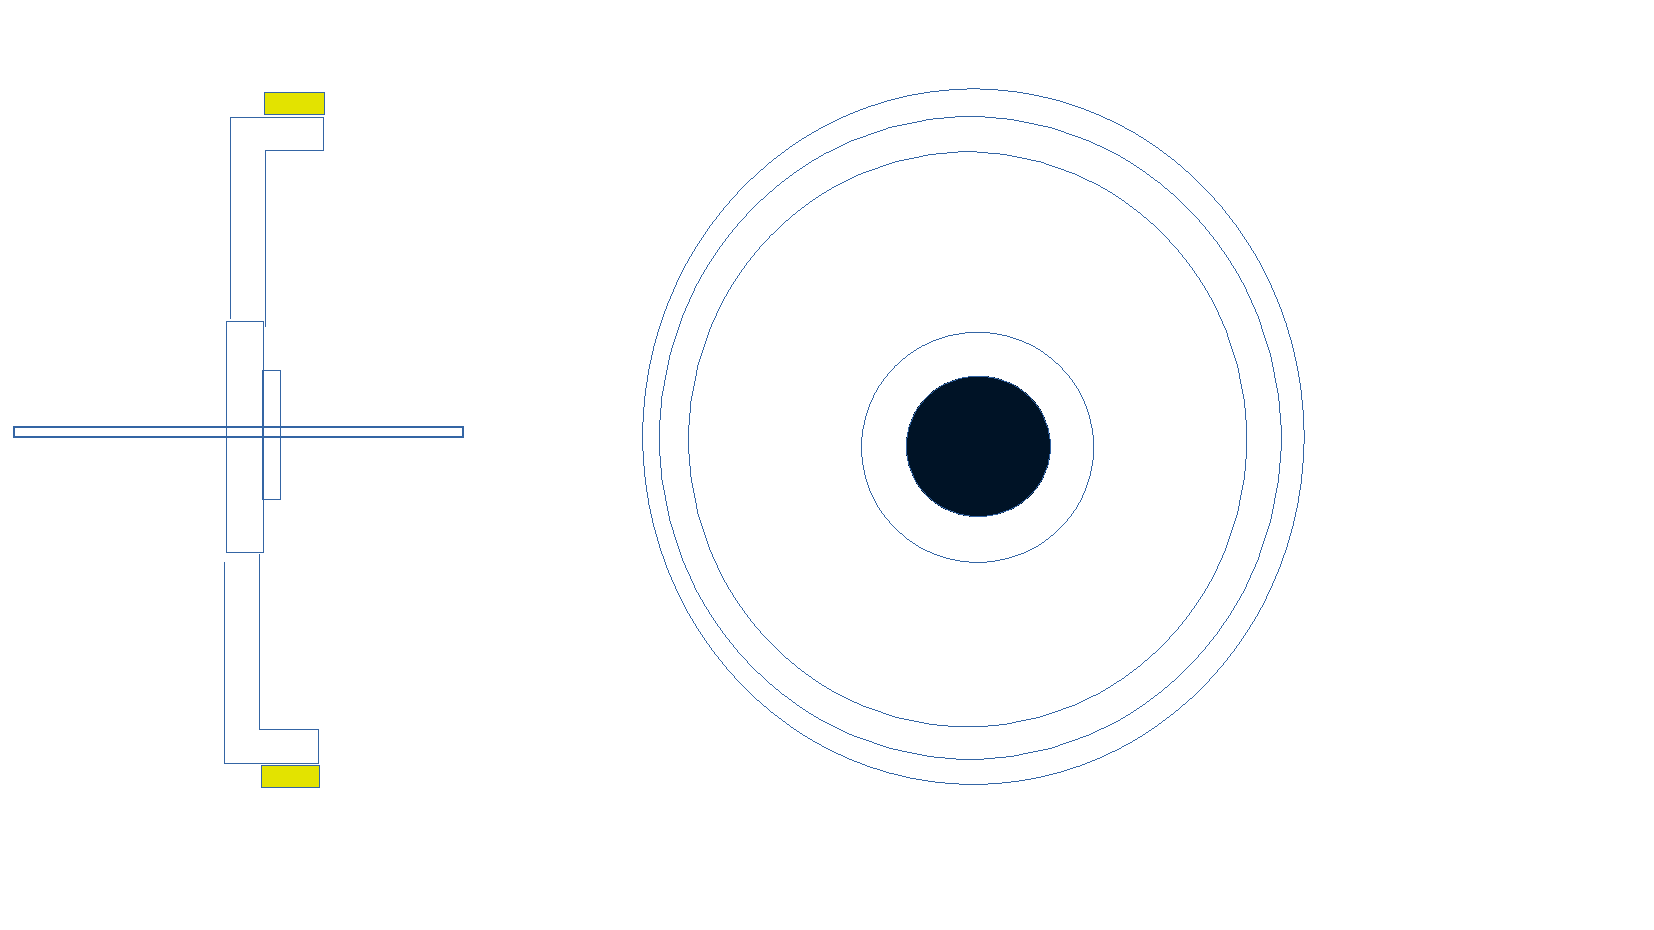
\includegraphics[width=0.95\textwidth]{pdf/degrader_geometry_001}
      }
    };
    % \node [text width=8cm, scale=1.0] at (14.5,0.5) {$\mu_B$, expected background mean};
    % \node [text width=8cm, scale=1.0, rotate={90}] at (1.5,7.5) { $S_{D}$, ``discovery'' signal strength  };
  \end{tikzpicture}
  \caption{
    \label{figure:degrader_geometry_001}
    Schematic view of the simulated degrader geometry
  }
\end{figure}

The considered degrader geometry is schematically shown in Figure~\ref{figure:degrader_geometry_001}.
A gold converter ring has the outer radius $R_{out}$ = 250mm, and the value of $R_{in}$ is defined
by the converter thickness.

From \piplusenu\ studies: the degrader disk thickness of 4 mm Ti is close to optimal.
4mm of Ti translates into the total amount of material of $1.8 g/cm^2$, about twice that
of the stopping target.
\begin{itemize}
\item
  9mm CH2 + 1.0mm Pb: : 2.0 $g/cm^2$   .. $\pi*15^2*(0.9*0.95 + 0.08*11.34): \simeq 2 g/cm^2$
\item
   9mm CH2 + 0.8mm Pb: : $1.76 g/cm^2$
 \item
   reduce the outer radius of the degrader disk - don't need 15 cm
 \item
   CH2 disk R=14 cm, weight        : $0.9*0.95*\pi*14^2$ = 526 gr \\
   Pb  foil R=10cm thickness 0.8mm : 0.08*11.34*314    = 285 gr \\
   total                           : 811 gr
\end{itemize}

To make sure that $e^+$ and $e^-$ do not cross the converter foil multiple times,
the converter is moved downstream by 1cm with respect to the degrader disk.

The converter foil could be supported by a carbon foam disk surrounding the degrader.
A potentially more attractive alternative could be to support the converter placed
on a thin carbon foam ring, on the OPA. That would allow to increase the acceptance
by increasing the width of the converter ring.

{\red The impact on the CE acceptance should be minimal, but needs to be quantified.}

As the $\gamma \to e^+e^-$ acceptance is proportional to the width of the converter ring,
making it 3cm wide instead of 1 cm wide would increase the acceptance by a factor of x3.

%%%%%%%%%%%%%%%%%%%%%%%%%%%%%%%%%%%%%%%%%%%%%%%%%%%%%%%%%%%%%%%%%%%%%%%%%%%%%%
\subsection{pion stops}

Momentum and time:

\begin{figure}[H]
  \begin{tikzpicture}
    \node[anchor=south west,inner sep=0] at (0,0.) {
      % \node[shift={(0 cm,0.cm)},inner sep=0,rotate={90}] at (0,0) {}
      % \makebox[\textwidth][c] {
        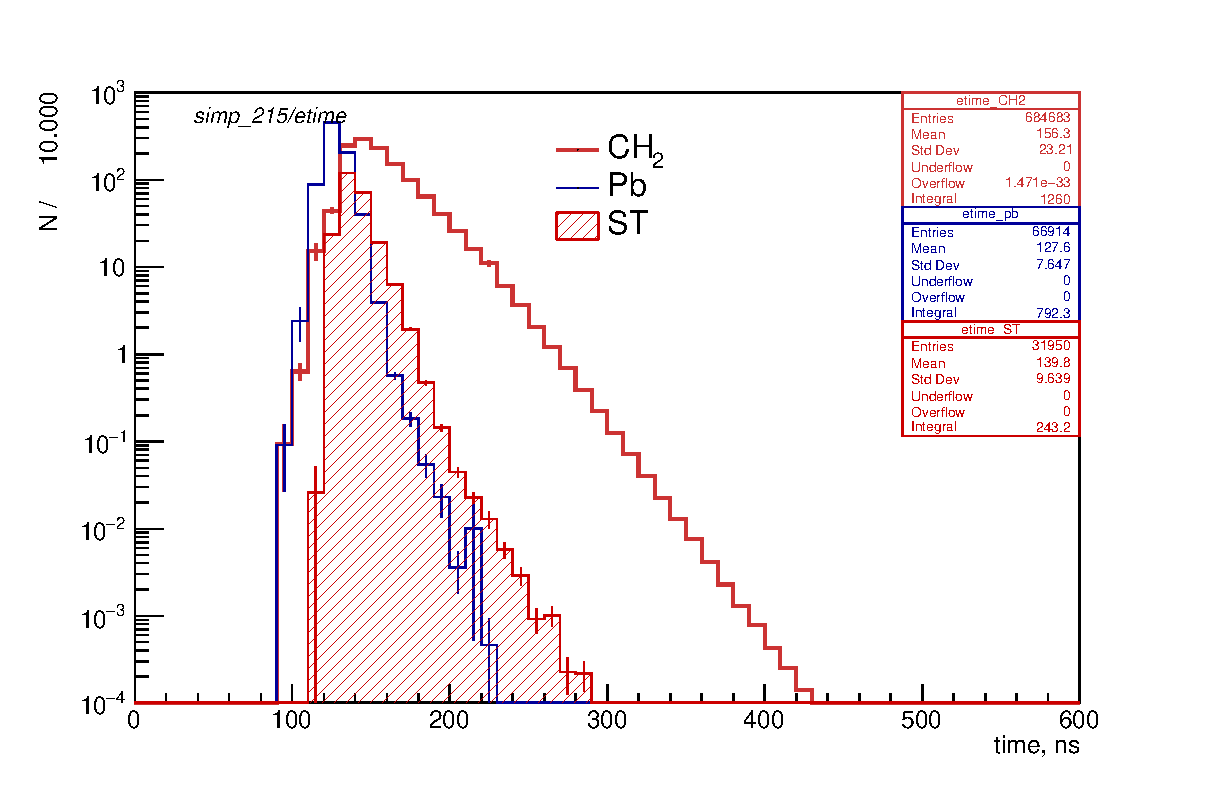
\includegraphics[width=0.5\textwidth]{png/figure_00021}
      % }
    };
    \node[anchor=south west,inner sep=0] at (10,0.) {
      % \node[shift={(0 cm,0.cm)},inner sep=0,rotate={90}] at (0,0) {}
      % \makebox[\textwidth][c] {
        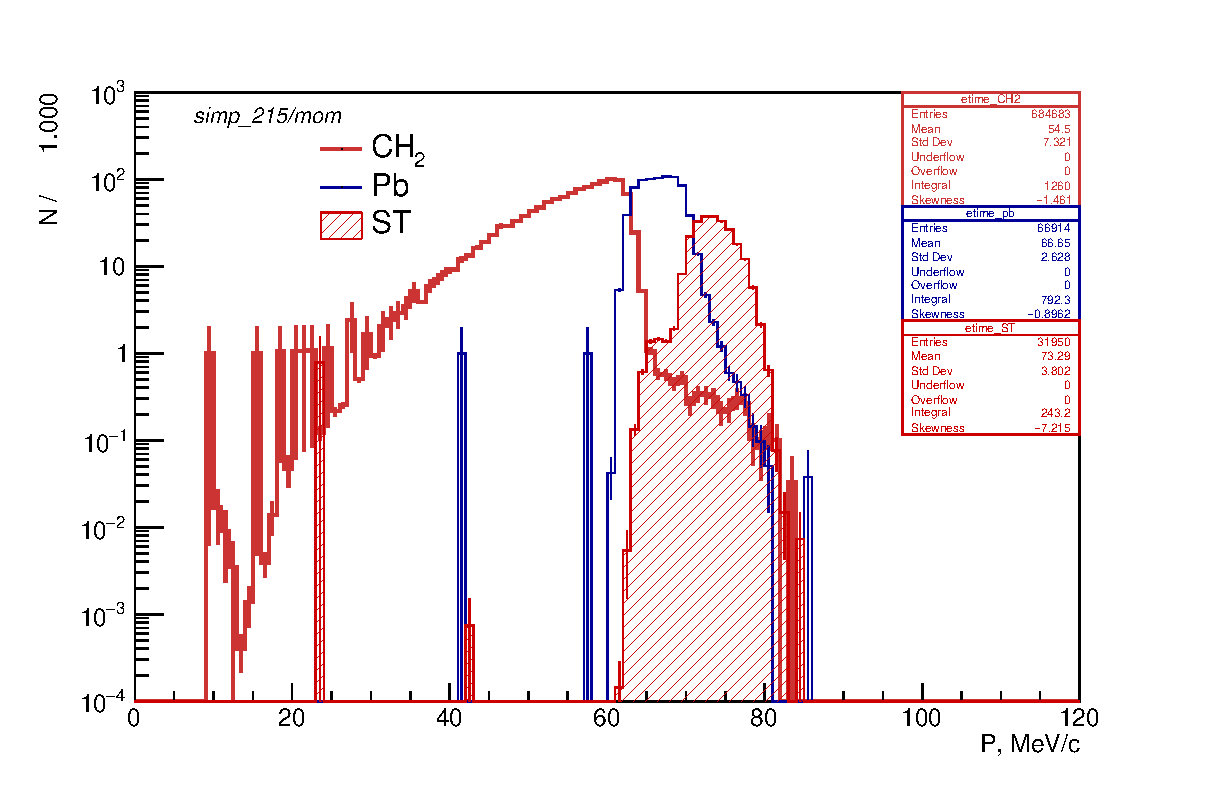
\includegraphics[width=0.5\textwidth]{png/figure_00022}
      % }
    };
    % \node [text width=8cm, scale=1.0] at (14.5,0.5) {$\mu_B$, expected background mean};
    % \node [text width=8cm, scale=1.0, rotate={90}] at (1.5,7.5) { $S_{D}$, ``discovery'' signal strength  };
  \end{tikzpicture}
  \caption{
    \label{figure:sum_mom_vd13}
    Stopped pions: distributions of momentum and time
  }
\end{figure}


The correlation between the vertical position of stopped particles in the degrader and the particle momentum
on exit from the TS is shown in Figure ~\ref{figure:y_vs_p_deg}.

\begin{figure}[H]
  \begin{tikzpicture}
    \node[anchor=south west,inner sep=0] at (0,0.) {
      % \node[shift={(0 cm,0.cm)},inner sep=0,rotate={90}] at (0,0) {}
      %\makebox[\textwidth][c] {
        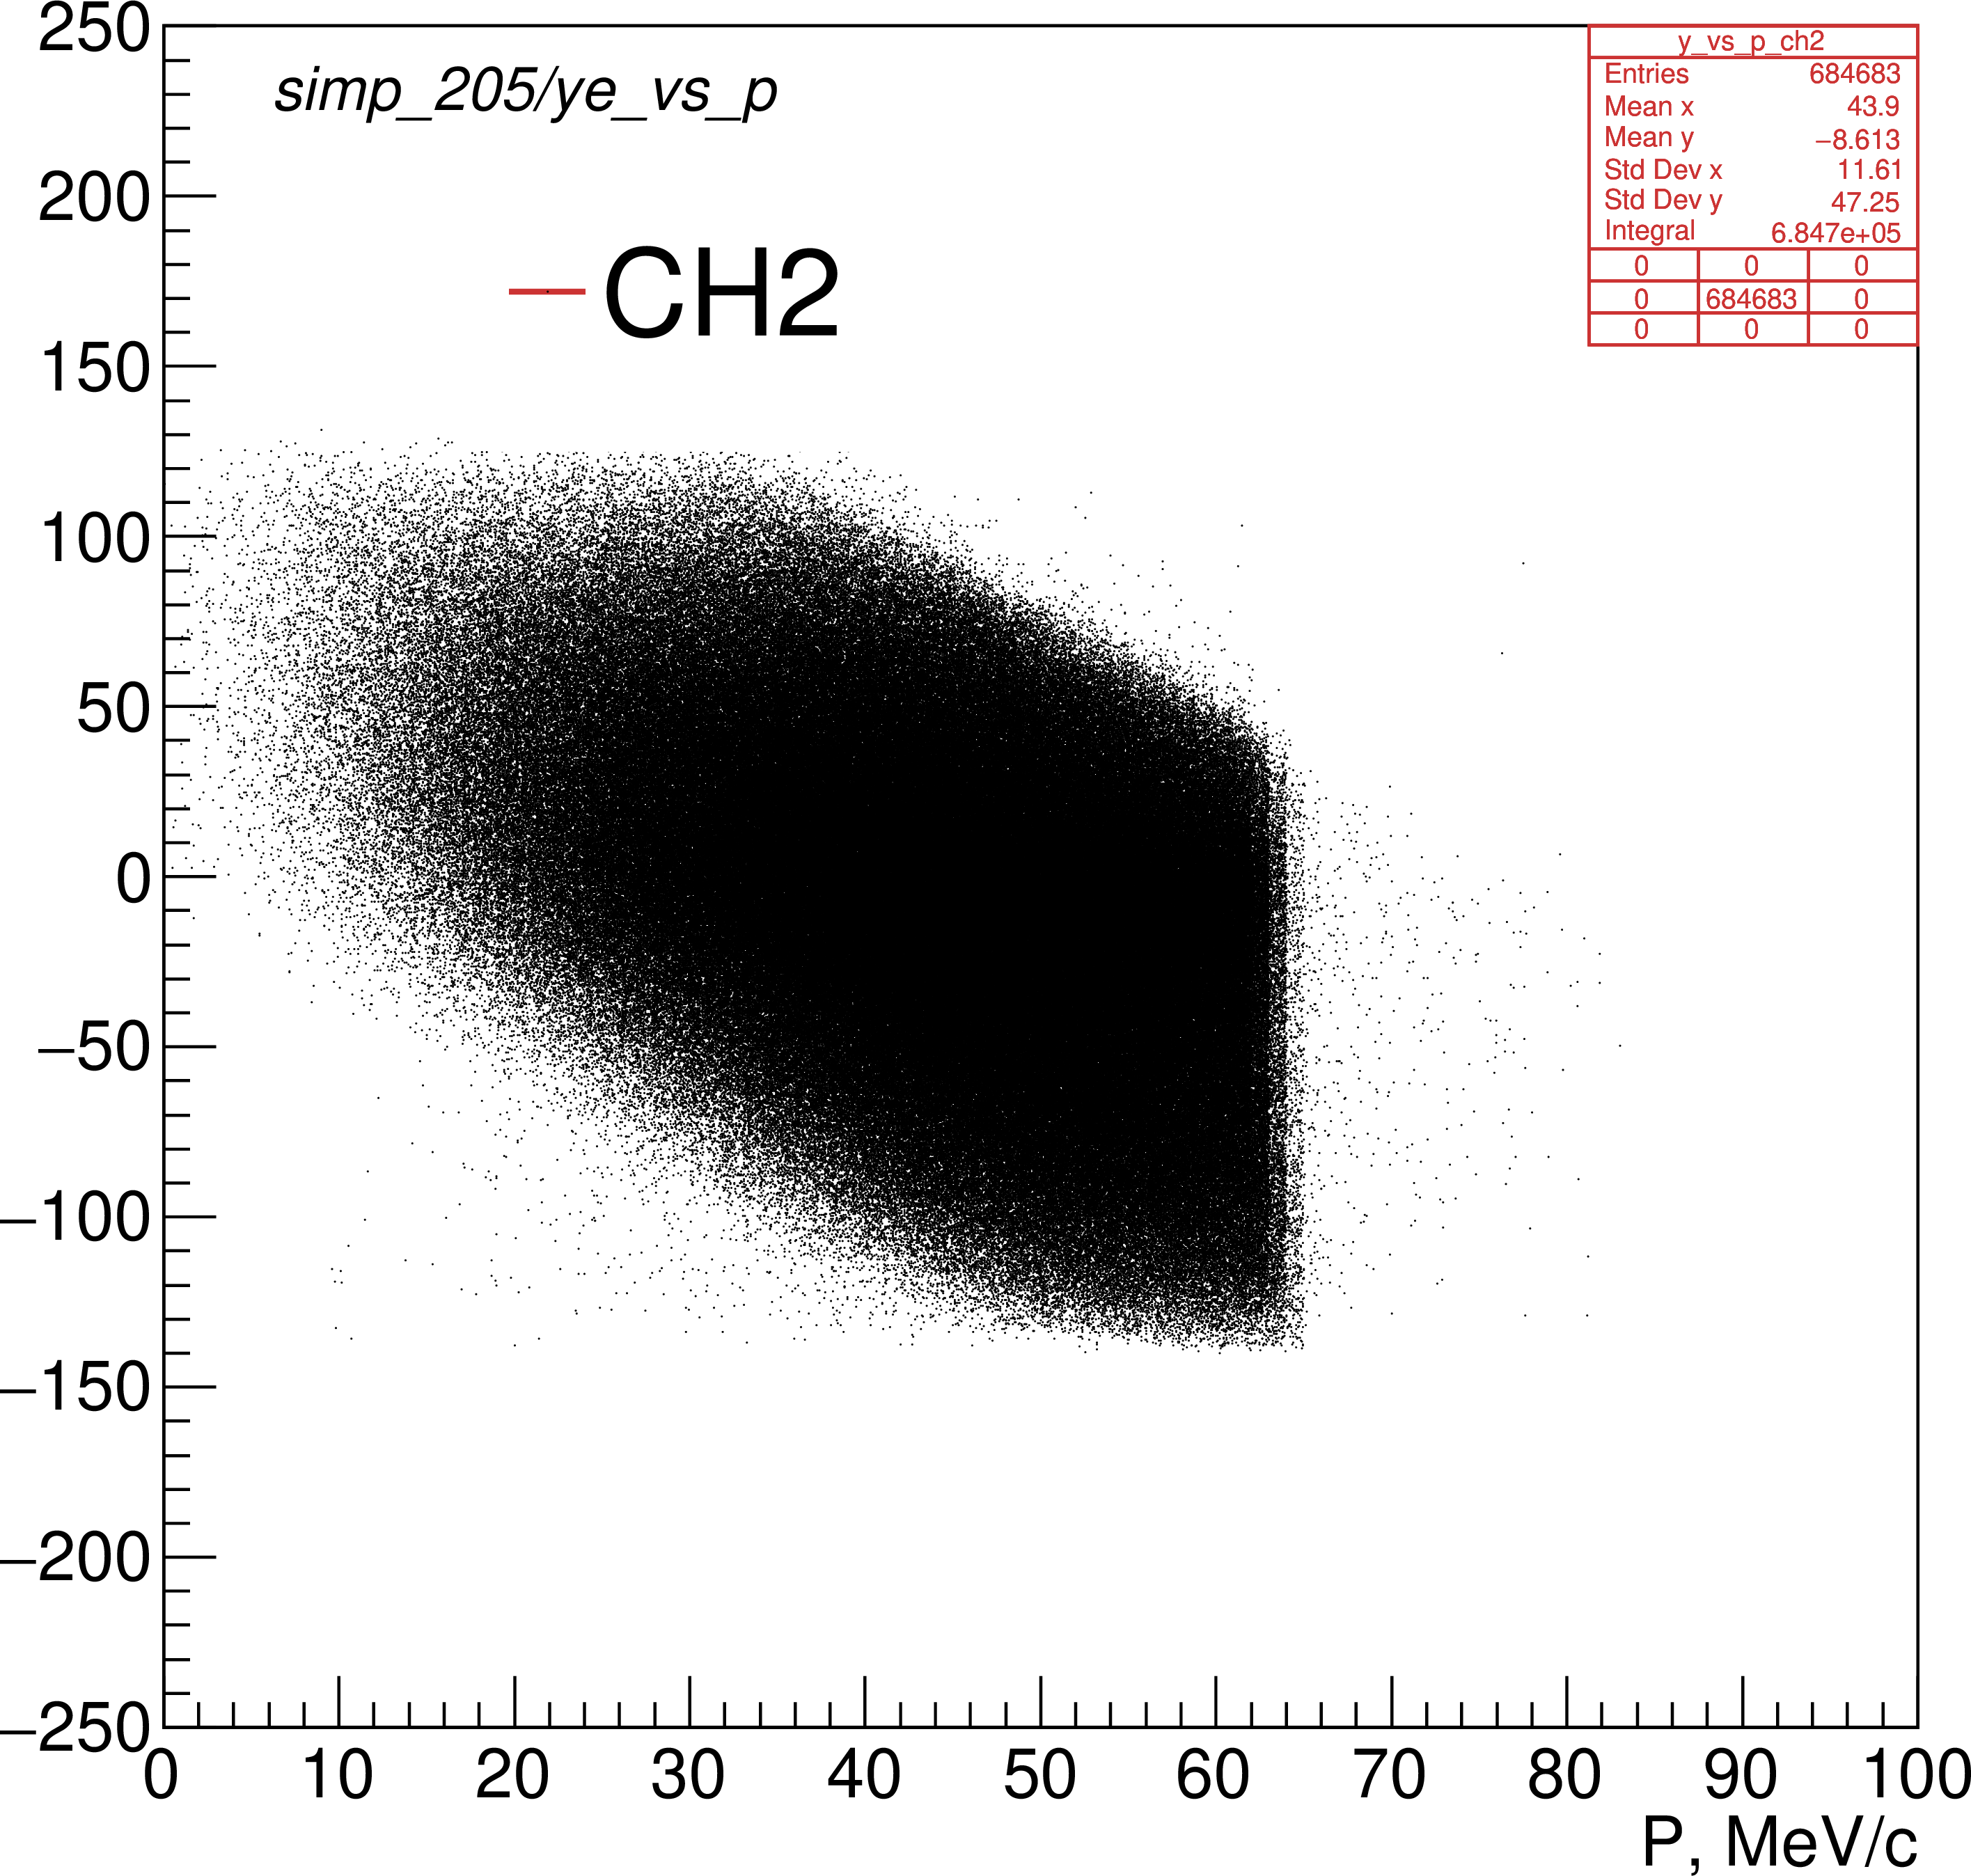
\includegraphics[width=0.5\textwidth]{png/figure_00036}
      %}
    };
    \node[anchor=south west,inner sep=0] at (10.,0.) {
      % \node[shift={(0 cm,0.cm)},inner sep=0,rotate={90}] at (0,0) {}
      % \makebox[\textwidth][c] {
      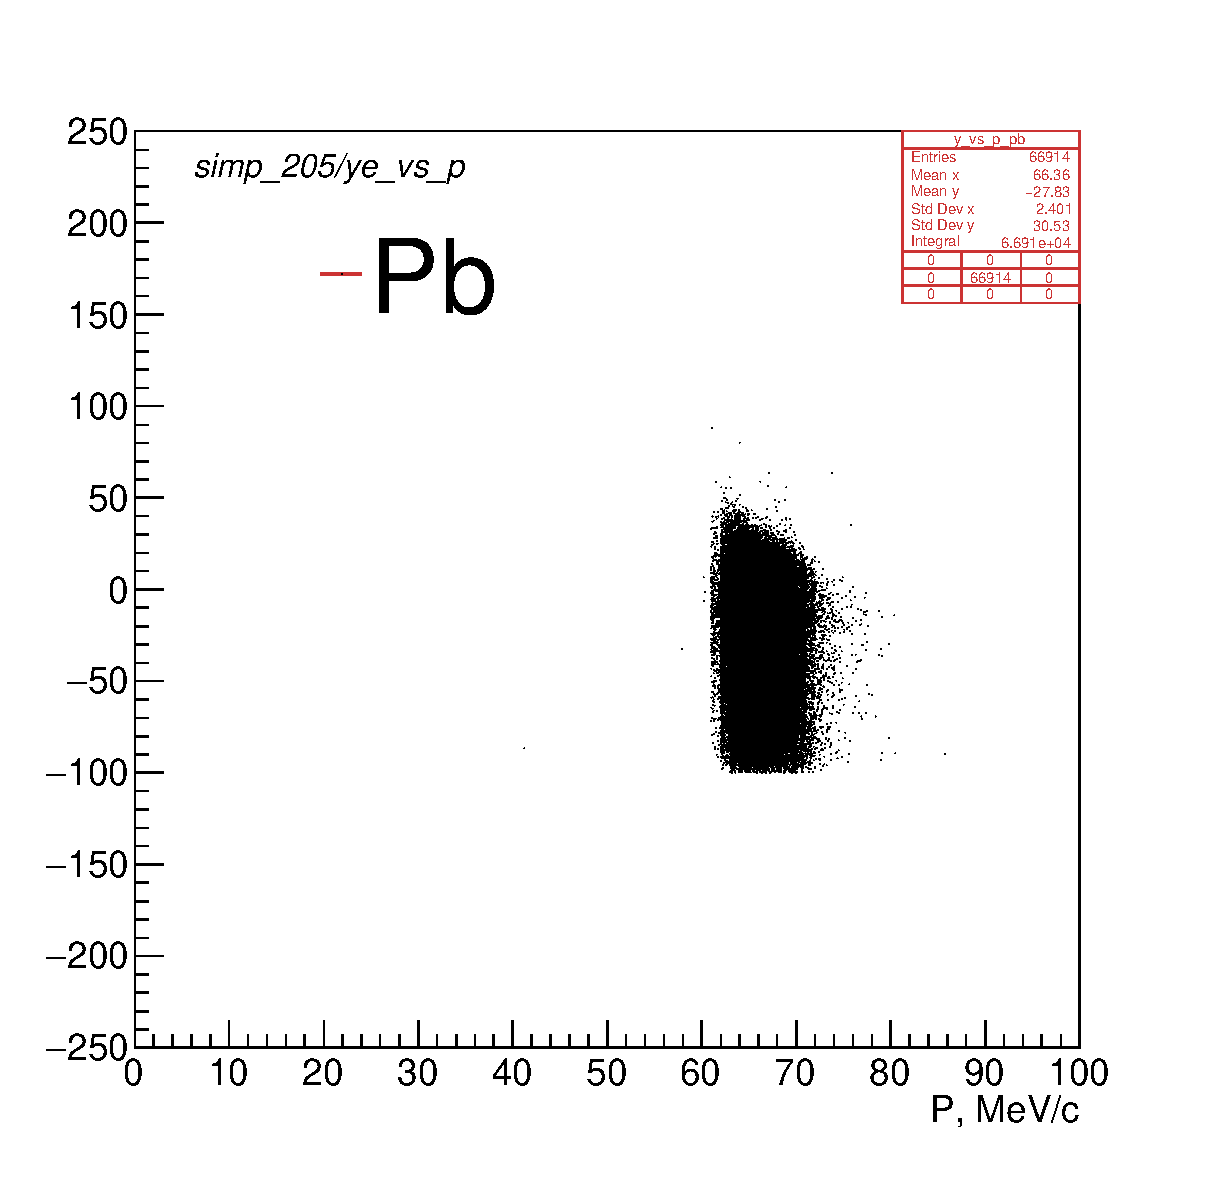
\includegraphics[width=0.5\textwidth]{png/figure_00037}
      %} 
    };
    % \node [text width=8cm, scale=1.0] at (14.5,0.5) {$\mu_B$, expected background mean};
    % \node [text width=8cm, scale=1.0, rotate={90}] at (1.5,7.5) { $S_{D}$, ``discovery'' signal strength  };
  \end{tikzpicture}
  \caption{
    \label{figure:y_vs_p_deg}
    Y(stop):P\@(DS entrance) for negative pions stopped in the $CH_2$ and Pb parts of the simulated degrader
  }
\end{figure}

The slowest, least energetic, pions stop in the CH2 disk. In most cases, those are also the ones arriving
to the DS later. Pions passing through the CH2 disk have momenta above 60 MeV/c. Due to the overcompensated
vertical drift in the TSu, their Y distribution is offset vertically in the negative direction -
see Figure ~\ref{figure:y_vs_x_st}. Y distribution of pions stopping in the ST is also offset towards
negative Y, but smeared by the pion motion.

\begin{figure}[H]
  \begin{tikzpicture}
    \node[anchor=south west,inner sep=0] at (0,0.) {
      % \node[shift={(0 cm,0.cm)},inner sep=0,rotate={90}] at (0,0) {}
      %\makebox[\textwidth][c] {
        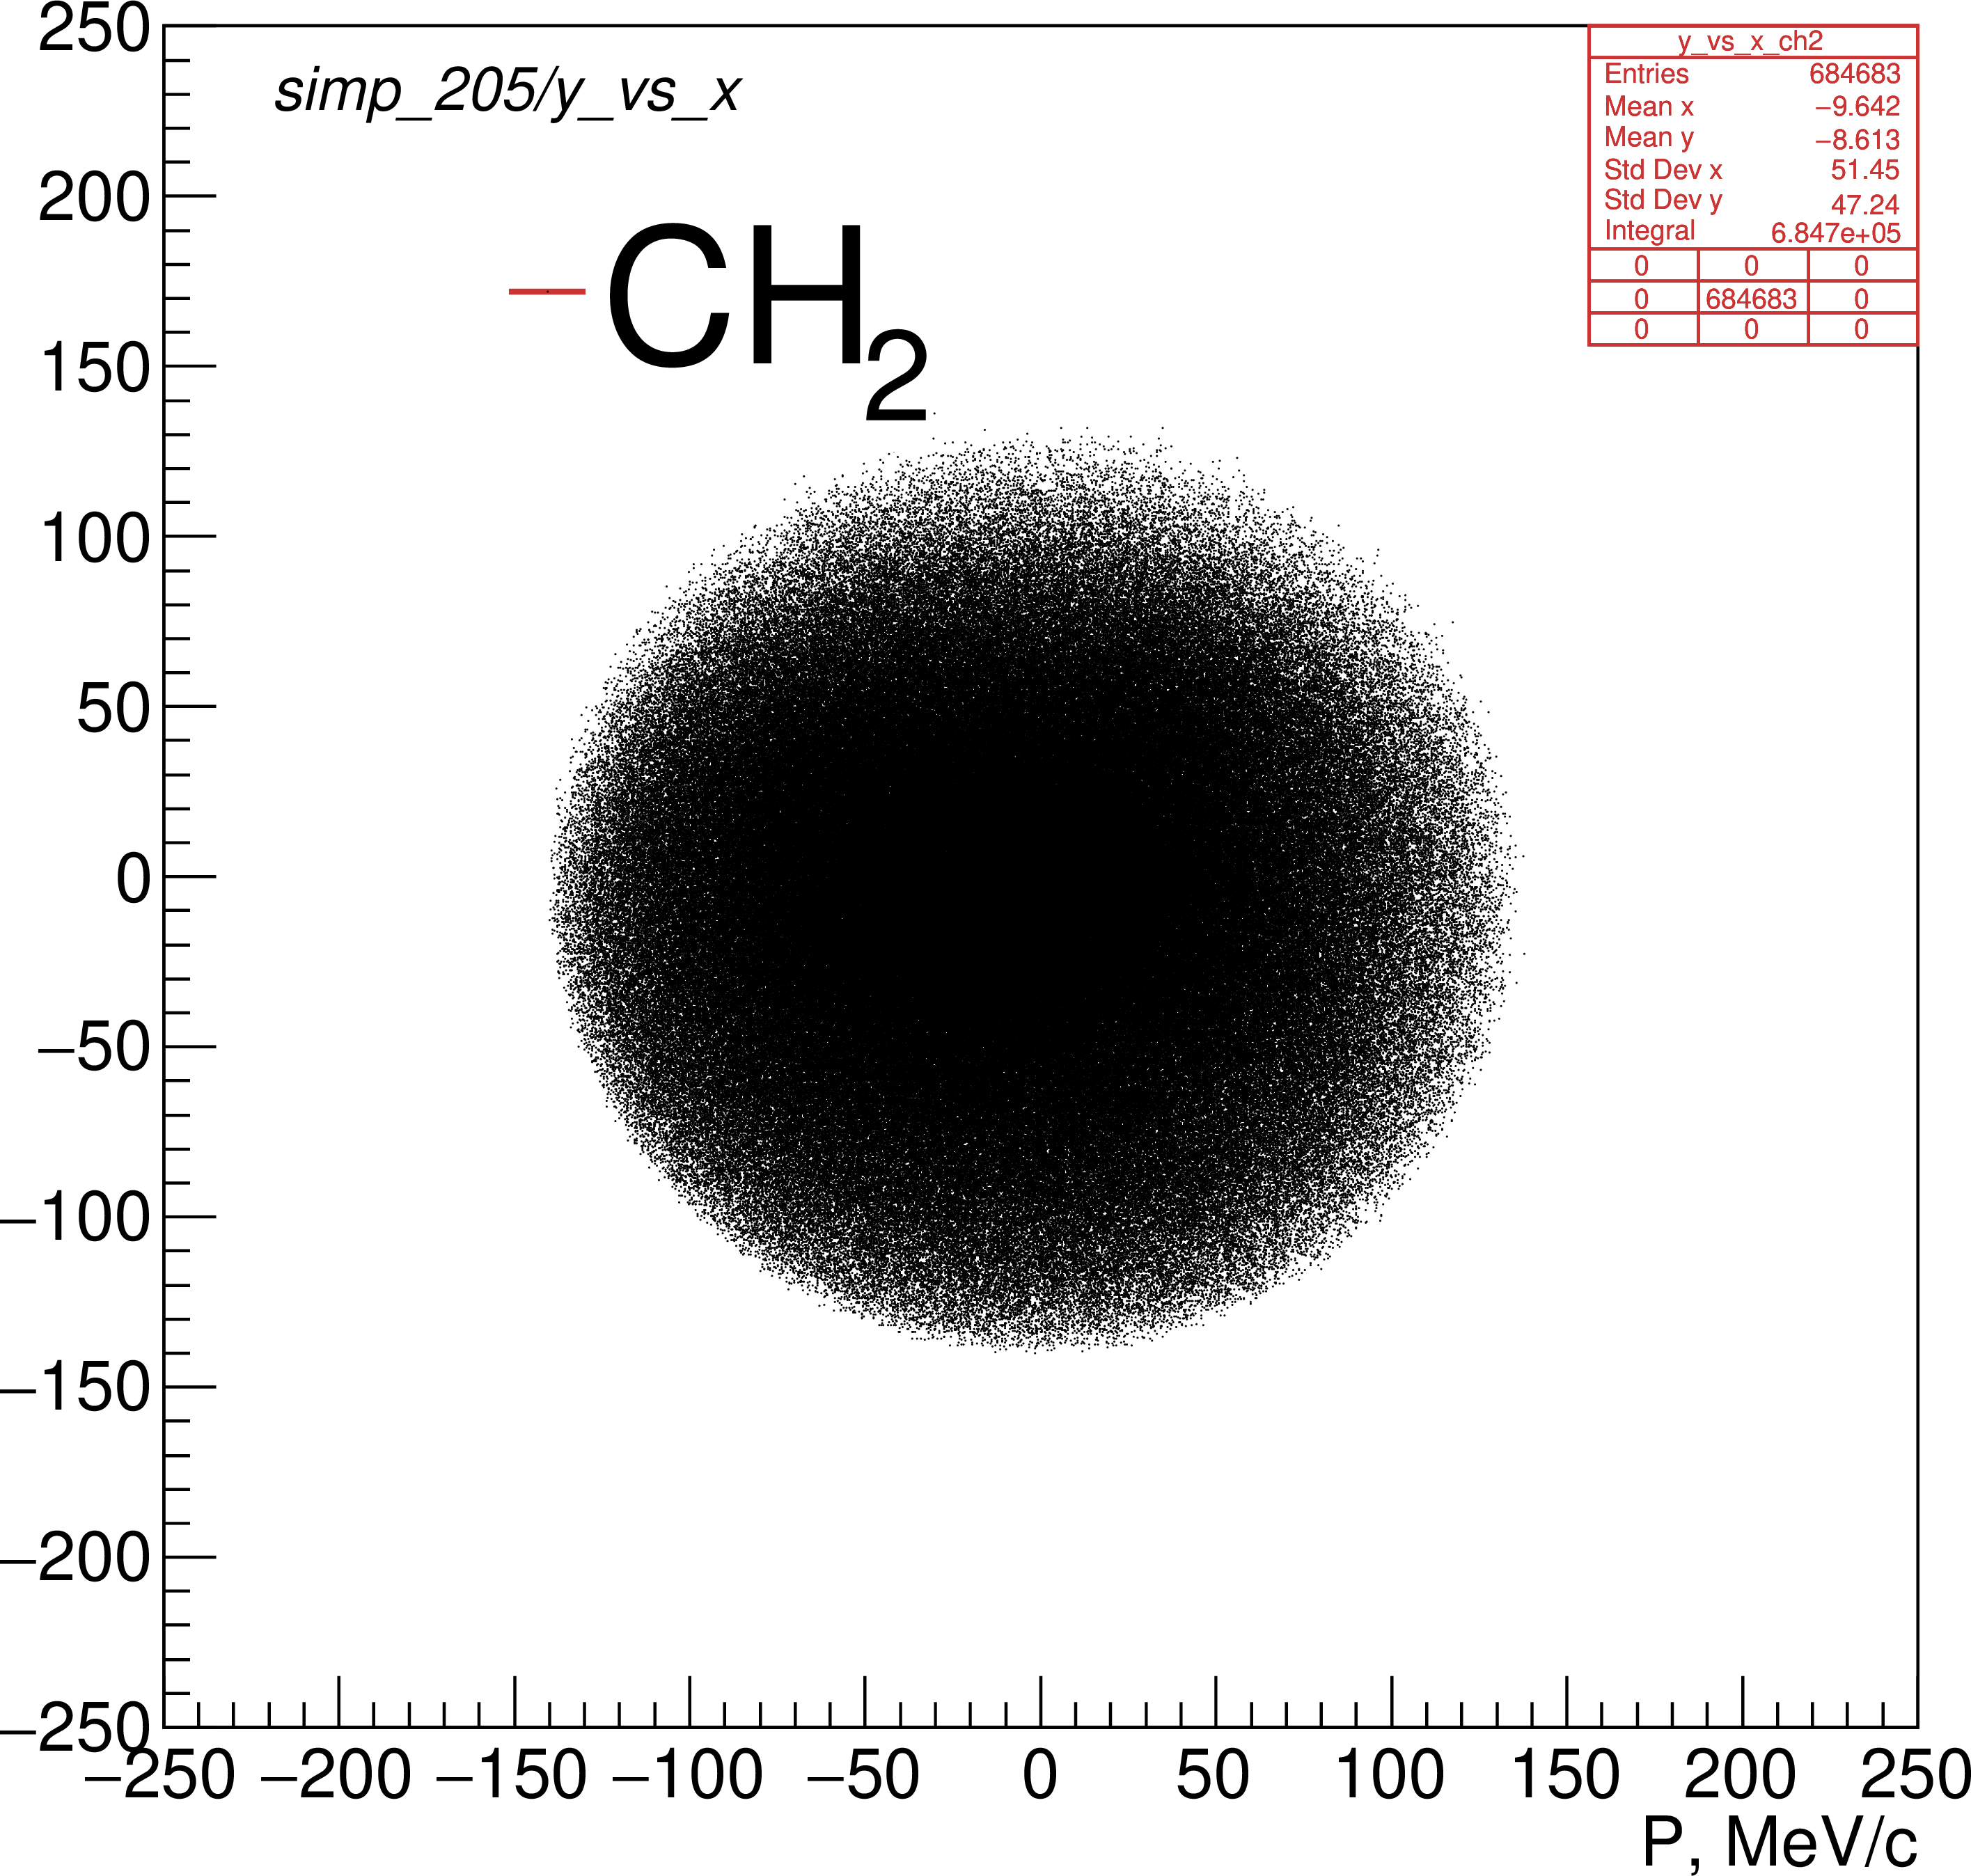
\includegraphics[width=0.5\textwidth]{png/figure_00034}
      %}
    };
    \node[anchor=south west,inner sep=0] at (10.,0.) {
      % \node[shift={(0 cm,0.cm)},inner sep=0,rotate={90}] at (0,0) {}
      %\makebox[\textwidth][c] {
        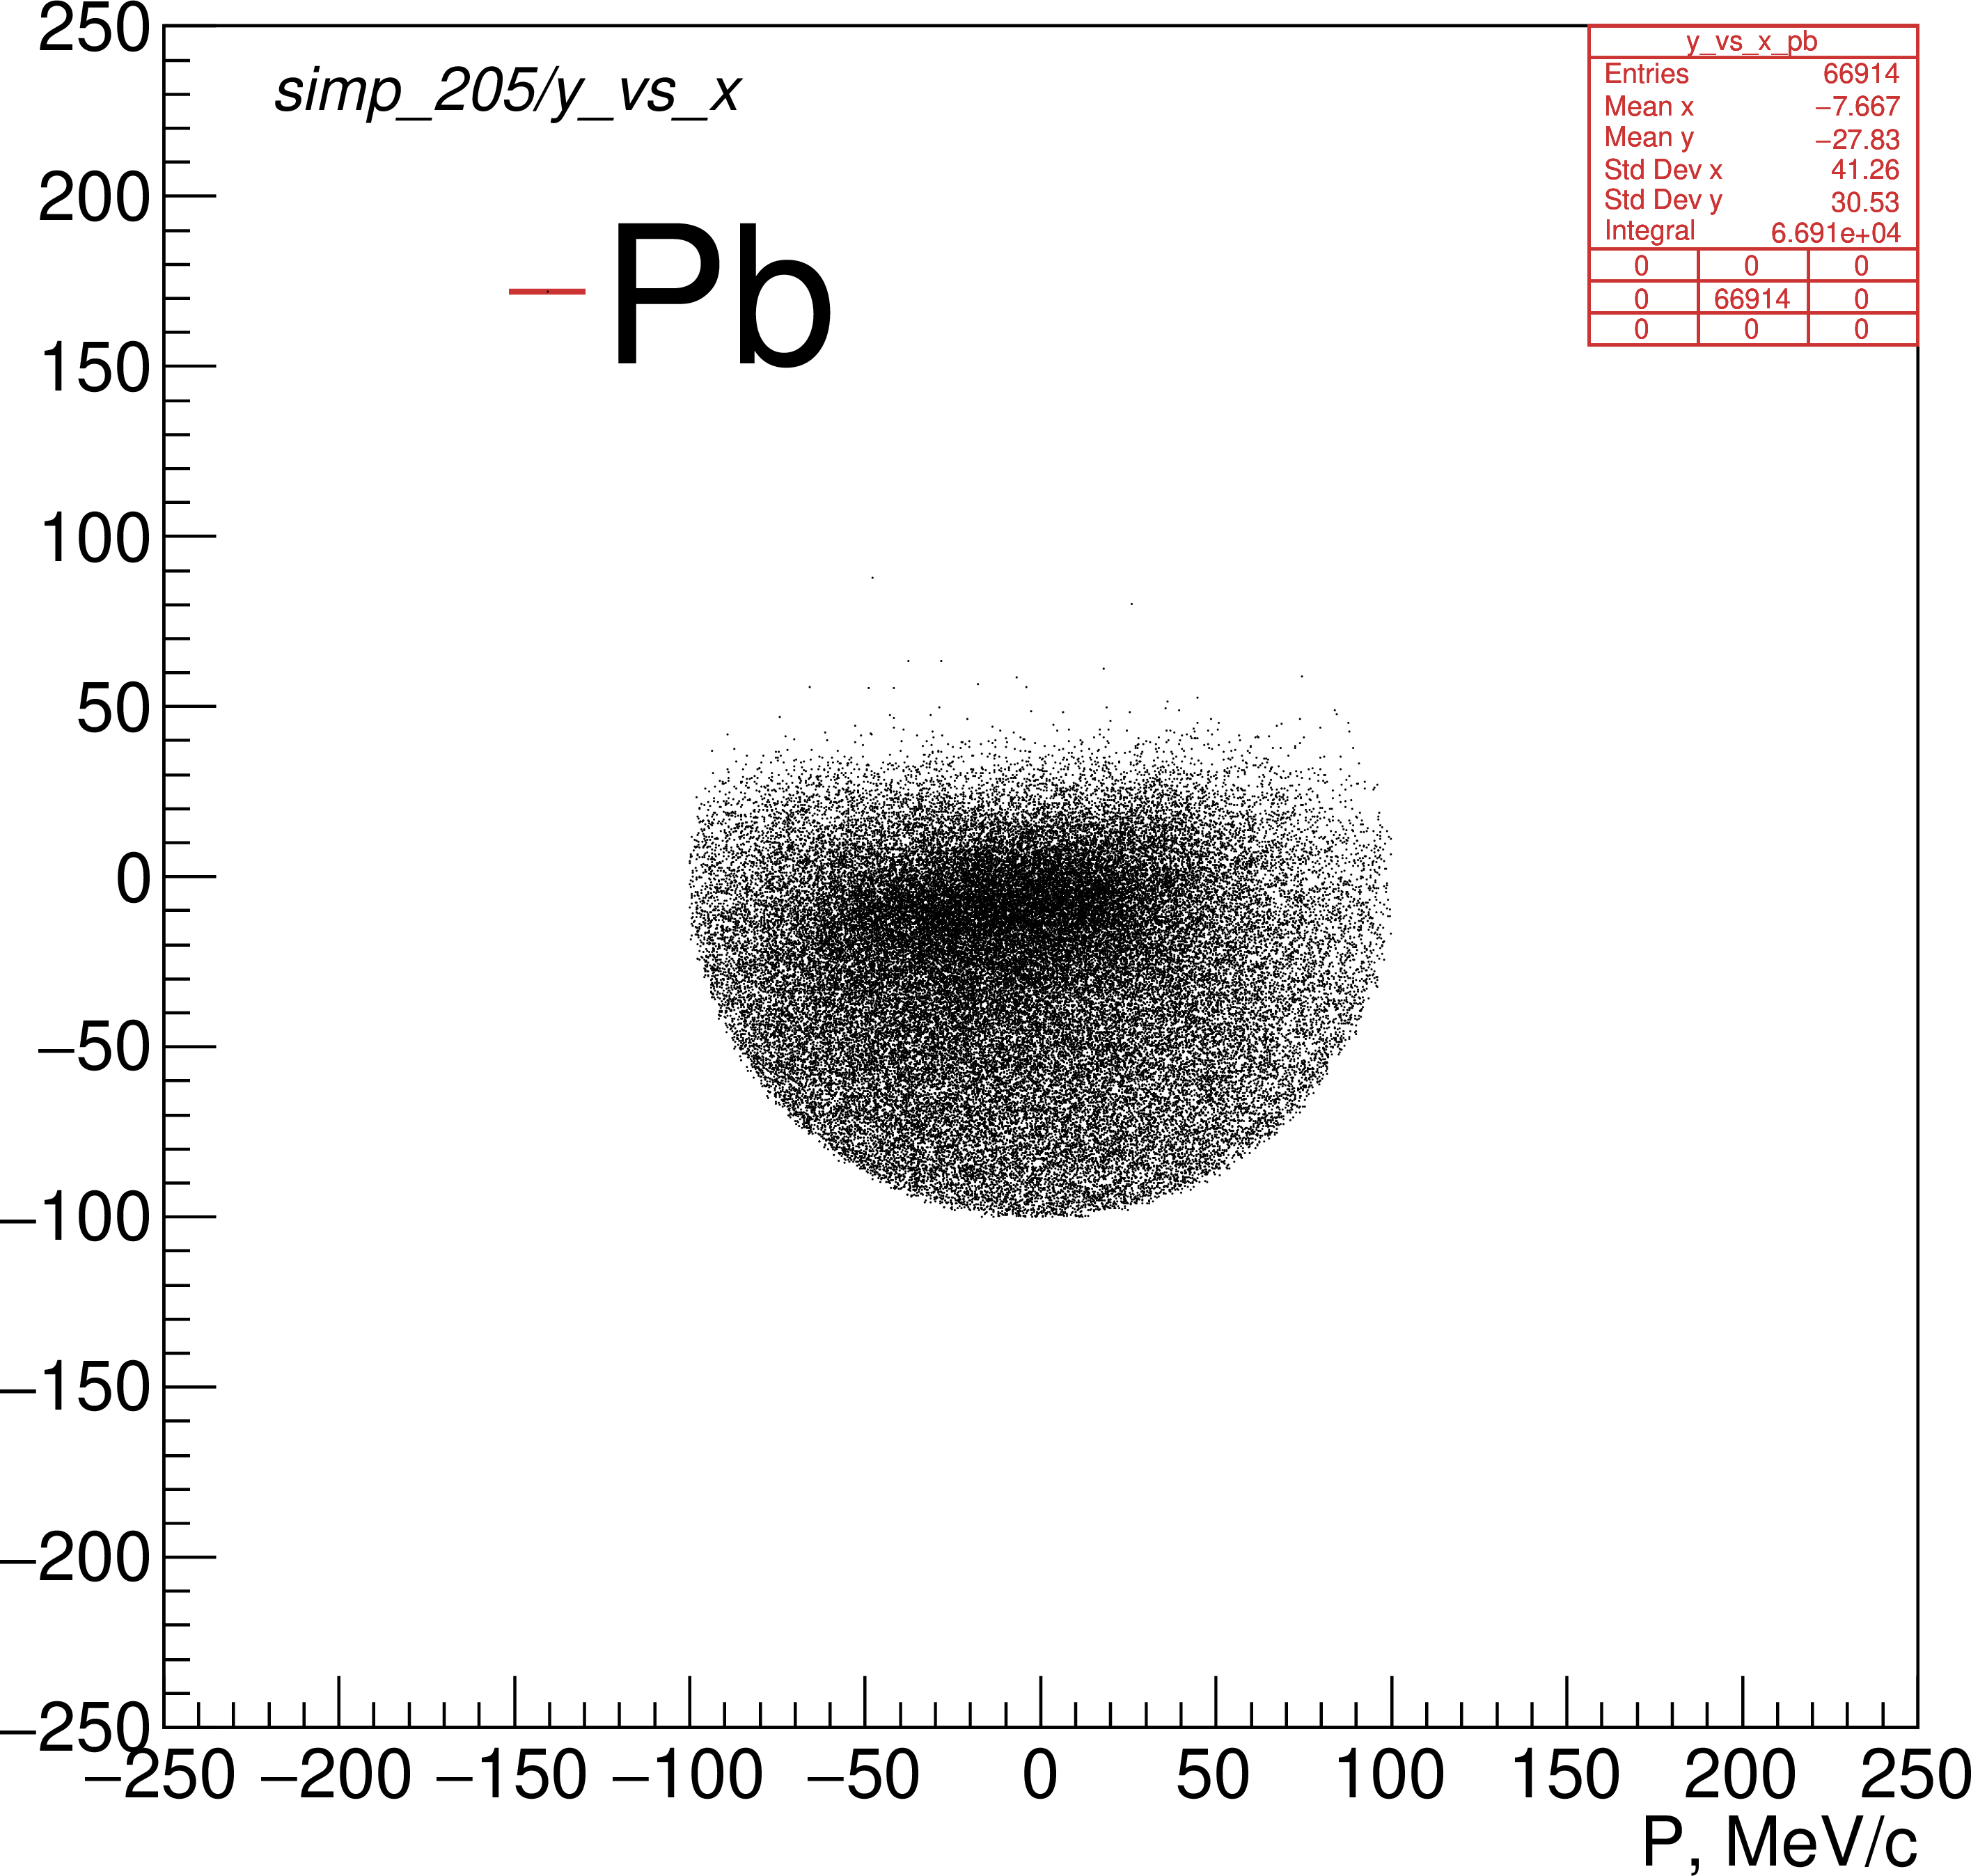
\includegraphics[width=0.5\textwidth]{png/figure_00035}
      %}
    };
    \node[anchor=south west,inner sep=0] at (0,-10.) {
      % \node[shift={(0 cm,0.cm)},inner sep=0,rotate={90}] at (0,0) {}
      % \makebox[\textwidth][c] {
        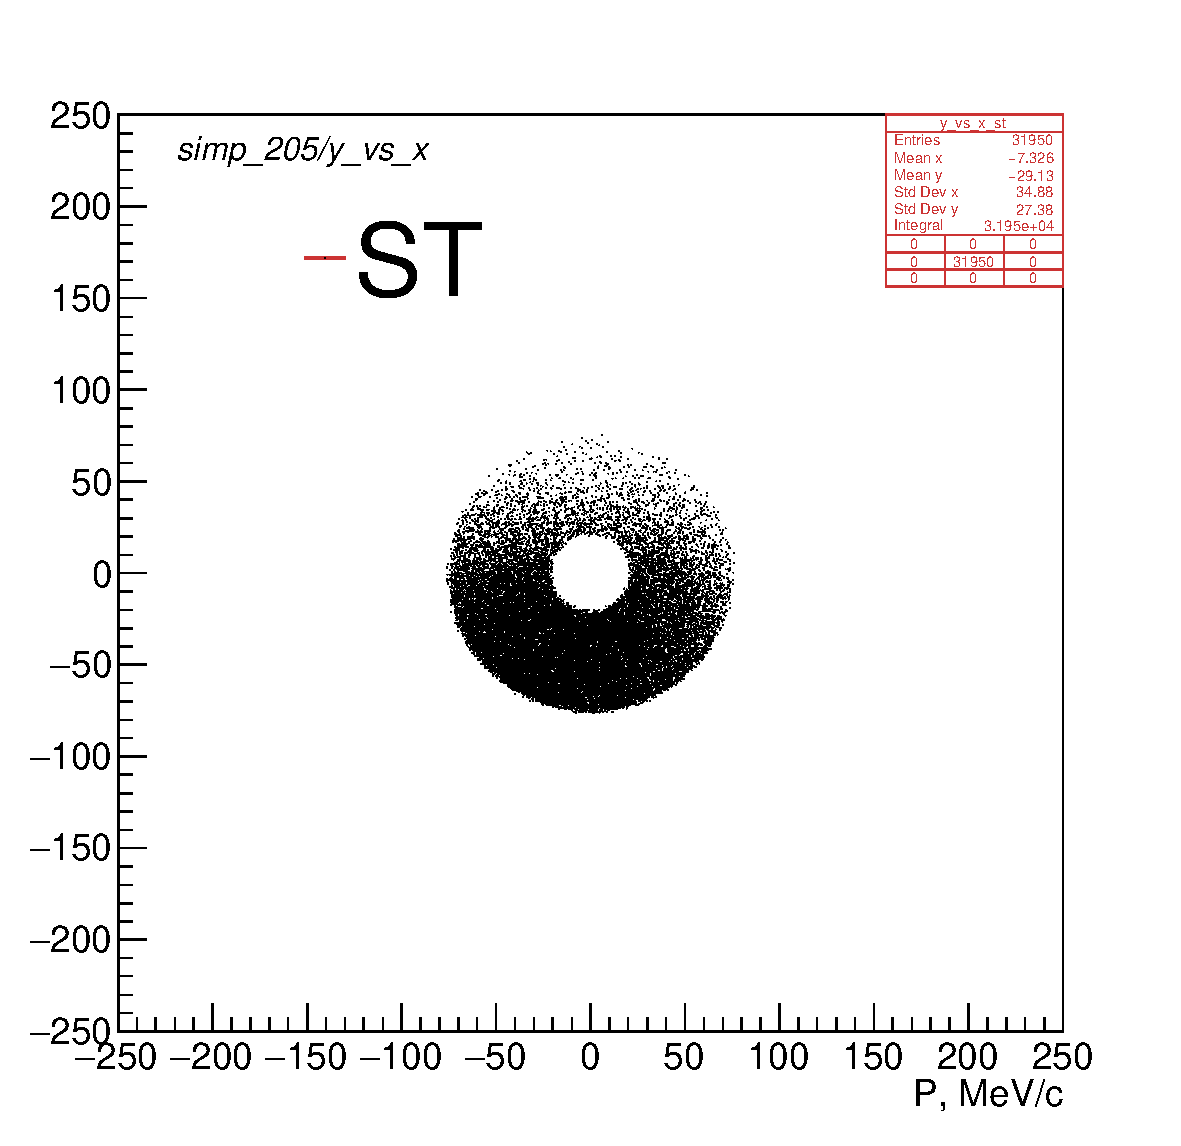
\includegraphics[width=0.5\textwidth]{png/figure_00031}
      % }
    };
    % \node [text width=8cm, scale=1.0] at (14.5,0.5) {$\mu_B$, expected background mean};
    % \node [text width=8cm, scale=1.0, rotate={90}] at (1.5,7.5) { $S_{D}$, ``discovery'' signal strength  };
  \end{tikzpicture}
  \caption{
    \label{figure:y_vs_x_st}
    Y(stop):X(stop) for pions stopped in the CH2, Pb, and ST
  }
\end{figure}


%%% Local Variables:
%%% mode: latex
%%% TeX-master: t
%%% End:
